\documentclass[conference]{IEEEtran}
\IEEEoverridecommandlockouts
\setlength{\columnsep}{10mm}
% The preceding line is only needed to identify funding in the first footnote. If that is unneeded, please comment it out.
\usepackage{cite}
\usepackage{amsmath,amssymb,amsfonts}
\usepackage{algorithmic}
\usepackage{graphicx}
\usepackage{booktabs}
\usepackage{subcaption}
\usepackage{textcomp}
\usepackage[dvipsnames]{xcolor}
\usepackage{hyperref}
\def\BibTeX{{\rm B\kern-.05em{\sc i\kern-.025em b}\kern-.08em
    T\kern-.1667em\lower.7ex\hbox{E}\kern-.125emX}}
\begin{document}

\title{Outperforming Morningstar Analysts: \\ Applying Enhanced LLMs to Financial Reports
%{\footnotesize \textsuperscript{*}Note: Sub-titles are not captured in Xplore and should not be used}
}

\author{\IEEEauthorblockN{1\textsuperscript{st} Jonas Gottal }
\IEEEauthorblockA{\textit{LMU Munich} \\
\textit{Department of Computer Science}\\
%City, Country \\
%email address or ORCID
}
\and
\IEEEauthorblockN{2\textsuperscript{nd} Mohamad Hgog}
\IEEEauthorblockA{\textit{LMU Munich} \\
\textit{Department of Computer Science}\\
%City, Country \\
%email address or ORCID
}
}

\maketitle

\begin{abstract}
This study examines financial analyst reports from Morningstar, revealing two key findings: firstly, analysts appear to select stocks arbitrarily, and secondly, they provide comprehensive textual justifications that enable informed decisions surpassing mere chance. We employ enhanced large language models to efficiently analyze the textual data, facilitating a broad exploration of various pre-trained models to identify the subtle underlying sentiment and extract more value from the reports than the experts themselves. The code is available at \href{https://github.com/trashpanda-ai/Advanced-Analytics-and-Machine-Learning}{github.com/trashpanda-ai}. %Describe Goal, data, method and results.
\end{abstract}

\begin{IEEEkeywords}
LLMs, PEFT, Adapters, Hugging Face, Finance
\end{IEEEkeywords}

\section{Introduction}
Many search for guidance in financial analyst reports for investment purpose. Especially during the COVID-19 pandemic, the number of retail traders has increased significantly. And Morningstar is one of the most popular platforms for financial reports that are widely used by both retail traders and professionals.

However, the question arises whether these reports are actually valuable or just an illusion of expertise. In this paper, we investigate the value of analyst reports and whether they can outperform the market. We hypothesize that the reports contain valuable information that can be extracted using enhanced large language models (LLMs) to outperform the market.
\section{Data} %Jonas %Report and financial market data.
Financial analysts provide detailed reports on single companies (equities), detailing their current situation and future prospects. These reports are based on a variety of factors, including their financial strength, economic moat and cost allocation. The reports also contain a rating and a fair price estimate. 

\subsection{Data description}%Jonas
The data is retrieved from \href{https://www.morningstar.co.uk/uk/}{Morningstar} and contains the following columns:
\begin{itemize}    
    \item \texttt{ParseDate}: The date the information was retrieved.
  \item \texttt{Title}: The title of the analyst report.
  \item \texttt{CompanyName}: The name of the company. 
  \item \texttt{TickerSymbol}: The ticker symbol (without exchange information) of the underlying stock.
  \item \texttt{Rating}: The analyst rating of the stock.
  \item \texttt{ReportDate}: The date of the release of the report. 
  \item \texttt{AuthorName}: The name of the author of the report. 
  \item \texttt{Price}: The price of the stock declared in the report.
  \item \texttt{Currency}: The given currency of the price. 
  \item \texttt{PriceDate}: The date the price was retrieved from market data (Morningstar).
  \item \texttt{FairPrice}: The estimated fair price from the analyst.
  \item \texttt{Uncertainty}: The company's uncertainty quantified in 'Low', 'Medium', 'High' and 'Very High'.
  \item \texttt{EconomicMoat}: The ability to maintain competitive advantages quantified in 'Narrow' and 'Wide'.
  \item \texttt{CostAllocation}:  Decisions on investments categorized as 'Poor', 'Standard', and 'Exemplary'.
  \item \texttt{FinancialStrength}: Rating of the ability to make timely payments and fulfill obligations -- quantified in 'A', 'B', ... 'F'.
  \item \texttt{AnalystNoteDate}: The date of the analyst note.
  \item \texttt{AnalystNoteList}: The analyst note.
  \item \texttt{BullsList}: Arguments in favor of the company.
  \item \texttt{BearsList}: Arguments against the company.
  \item \texttt{ResearchThesisDate}: The date of the thesis.
  \item \texttt{ResearchThesisList}: Objective research thesis.
  \item \texttt{MoatAnalysis}: Added research on EconomicMoat.
  \item \texttt{RiskAnalysis}: Company's risk profile. 
  \item \texttt{CapitalAllocation}: Text on the CostAllocation. 
  \item \texttt{Profile}: Short text on the company profile.
  \item \texttt{FinancialStrengthText}: Short text on the financial strength of the company (conclusion).
\end{itemize}
The most important information for the application of LLMs is the textual data -- starting with \texttt{AnalystNoteList}, which we expect to have the most effective content due to its subjective tone. We also analyze more objective texts like \texttt{BullsList} and \texttt{BearsList} as well as \texttt{ResearchThesisList}, \texttt{MoatAnalysis}, \texttt{RiskAnalysis}, \texttt{CapitalAllocation}, \texttt{Profile} and \texttt{FinancialStrengthText}.
Since the target group of financial analyst reports is investors, we focus on the long term perspective and not on short-term speculation. Therefore, we look at the stock price development over a longer period. The data is retrieved from Yahoo Finance and contains the following columns: \texttt{Date, Open, High, Low, Close, Adj Close} and \texttt{Volume}. We base our target variable for the sentiment analysis on the \texttt{Adjusted Close} price.

\subsection{Data Preprocessing}%Jonas
Since we care about investment and not speculation, we pre-process the data to remove spurious spikes and other noise. We focus on the archetype of a good investment as shown in Figure~\ref{fig:preprocessing1} and ignore spurious spikes as shown in Figure~\ref{fig:preprocessing2} and Figure~\ref{fig:preprocessing3}. This means we consider the average performance within a certain time period -- here the maximum amount since the last report was released: 120 days. Inspired by the commonly used moving averages in mathematical finance \cite{Hull2021}, the preprocessing is done by calculating the average stock price over 120 days since publication and comparing it to the stock price at the time of the report. If the average stock price is higher\footnote{A sideway movement within a 2\% margin is not classified as ``higher''.} than the price at time of release, we label it as a good investment, otherwise as a bad investment. This is our binary target variable for the following analysis.

\begin{figure}[h!]
    \centering
    \begin{subfigure}{.33\linewidth}
        \centering
        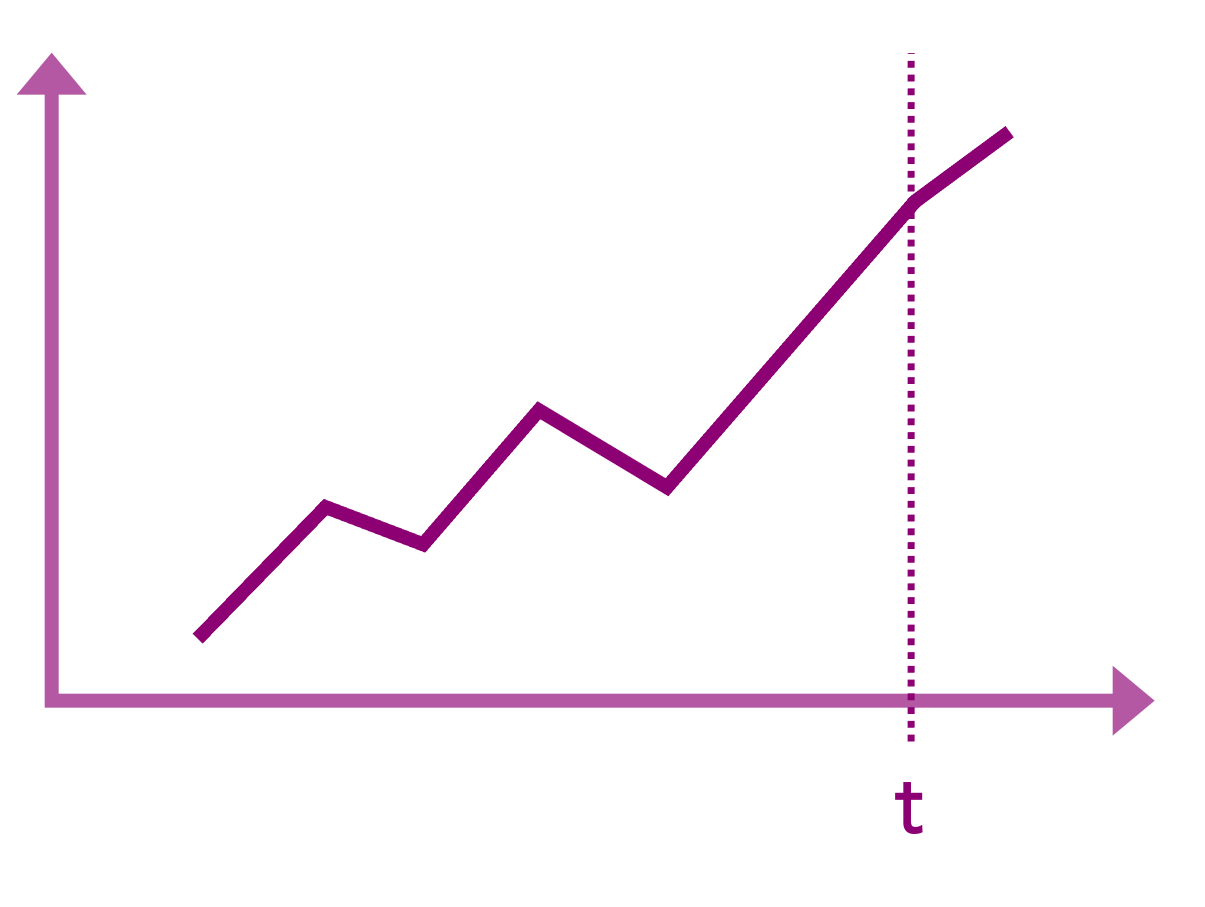
\includegraphics[width=\linewidth]{../5. report/pictures/preproccessing1.png}
        \caption{Archetype}
        \label{fig:preprocessing1}
    \end{subfigure}%
    \begin{subfigure}{.33\linewidth}
        \centering
        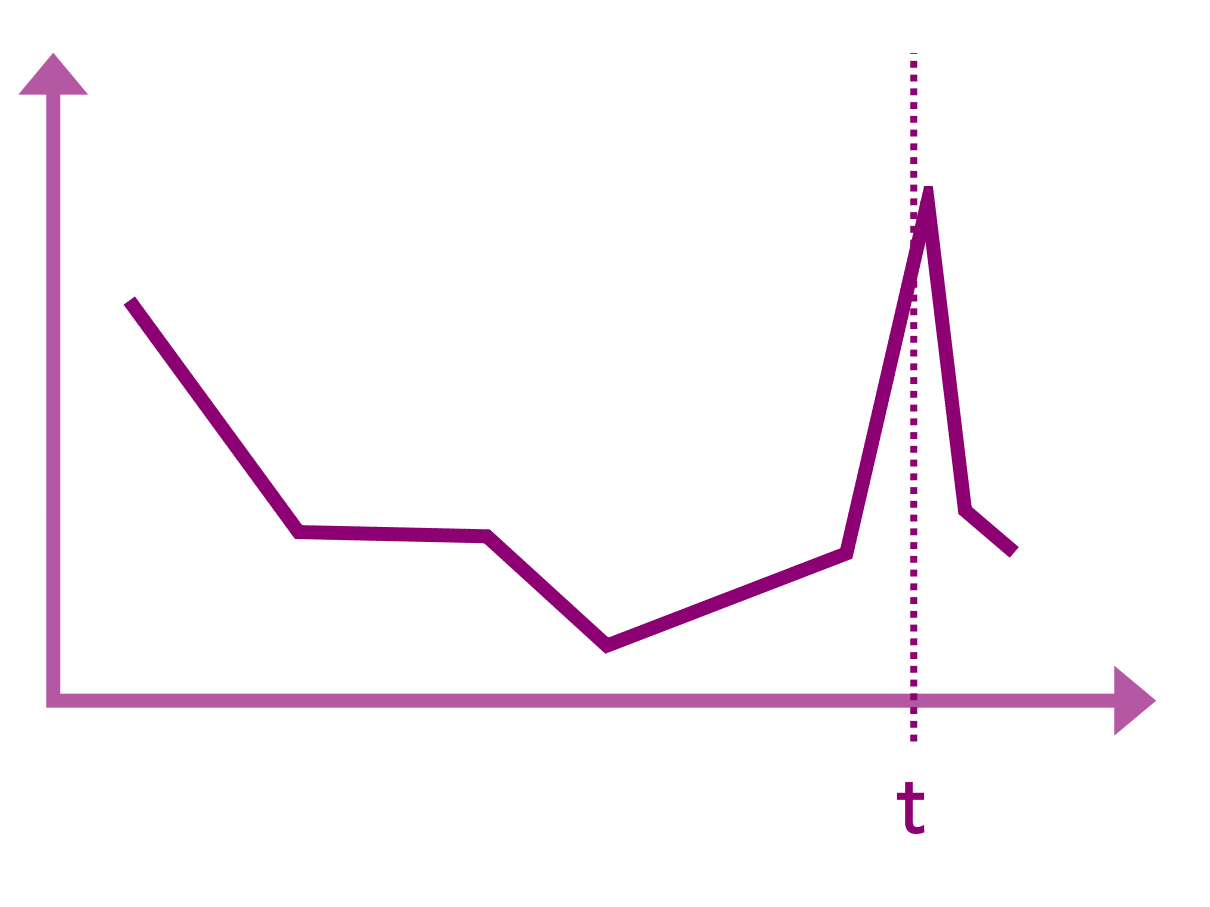
\includegraphics[width=\linewidth]{../5. report/pictures/preproccessing2.png}
        \caption{Pure luck}
        \label{fig:preprocessing2}
    \end{subfigure}%
    \begin{subfigure}{.33\linewidth}
        \centering
        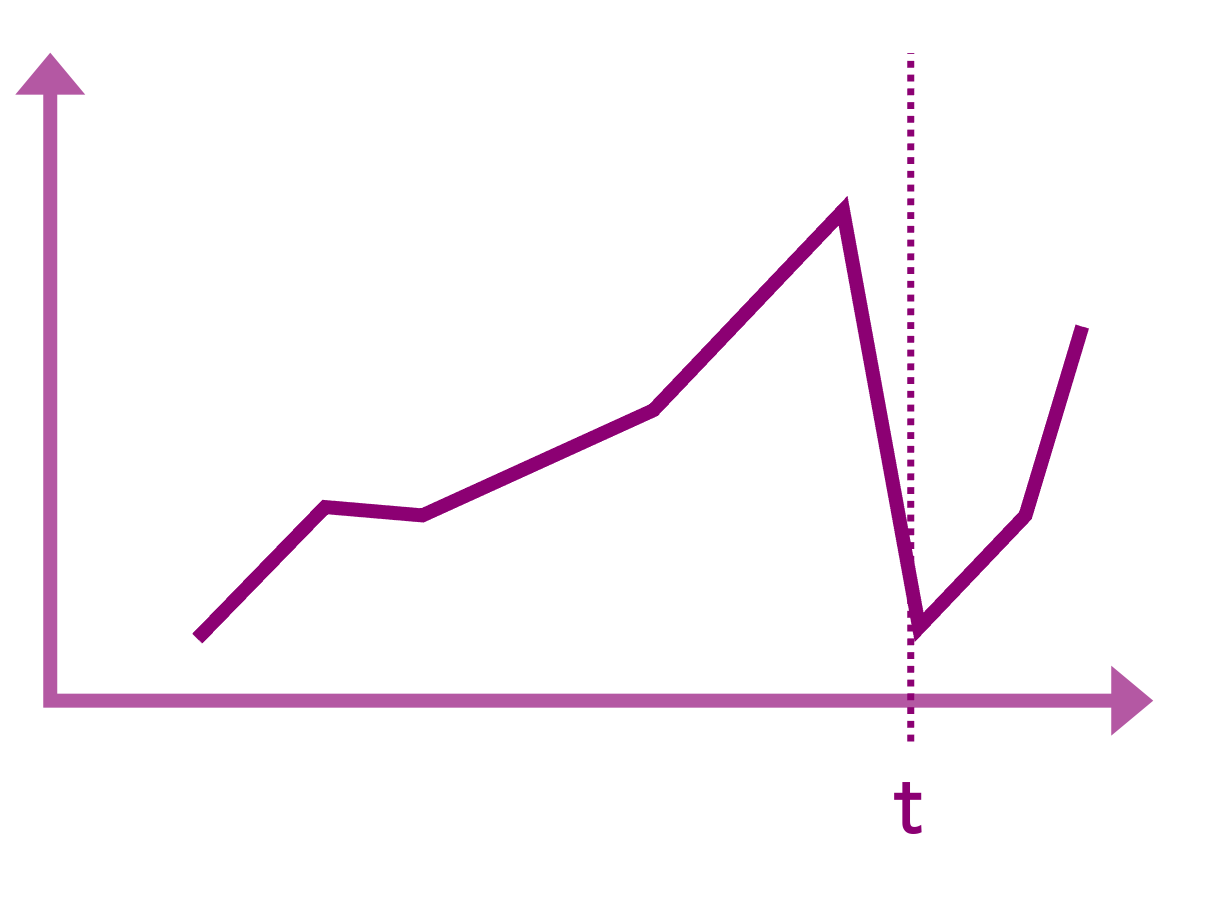
\includegraphics[width=\linewidth]{../5. report/pictures/preproccessing3.png}
        \caption{Bad luck}
        \label{fig:preprocessing3}
    \end{subfigure}
    \caption{Different stock developments as charts: Comparing the archetype of a good investment to spurious spikes (positive and negative). }
    \label{fig:preprocessing}
\end{figure}

The final data (1586 reports) is split into a training, development and test set with a ratio of 70:10:20 (1103, 165, 318). The training set is used to train the models, the development set to optimize the hyperparameters and the test set to evaluate the models.
\section{Foundations} %Mohamad
What are the foundations of our approach? What is the goal? Sentiment Classification.

\subsection{Transformer models}%Mohamad
Transformer models are a class of deep learning architectures that have revolutionized the field of natural language processing (NLP). These models, based on the encoder-decoder architecture, leverage self-attention mechanisms to process sequences of data in parallel and capture complex dependencies across the sequence. The encoder maps an input sequence of symbol representations $(x_1, \ldots, x_n)$ to a continuous representation $\mathbf{z}=(z_1, \ldots, z_n)$. The decoder generates an output sequence $(y_1, \ldots, y_m)$ from $\mathbf{z}$, using a method that is inherently auto-regressive, processing previous symbols to generate the next.

The backbone of the Transformer is the self-attention mechanism in both the encoder and decoder stacks, which allows each position in the sequence to attend to all positions in the previous layer of the model. Each encoder and decoder layer consists of multi-head self-attention mechanisms followed by position-wise fully connected feed-forward networks. Residual connections and layer normalization are employed around each sub-layer to facilitate the training of deep networks. Formally, each layer output can be described as:
\[
\text{Layer Output} = \text{LayerNorm}(x + \operatorname{Sublayer}(x))
\]
where $\operatorname{Sublayer}(x)$ represents the operations within the sub-layer itself.

\textbf{Self-attention} allows the model to weigh the importance of different words in the sequence irrespective of their positional distances. The attention function can be described as mapping a query and a set of key-value pairs to an output, where the output is a weighted sum of the values. The weight assigned to each value is computed by a compatibility function of the query with the corresponding key. The scaled dot-product attention is computed as:
\[
\operatorname{Attention}(Q, K, V) = \operatorname{softmax}\left(\frac{QK^T}{\sqrt{d_k}}\right)V
\]
where $Q$, $K$, and $V$ are the matrices representing queries, keys, and values, respectively, and $d_k$ is the dimensionality of the keys.

\textbf{Multi-head attention}, a pivotal extension of the basic attention mechanism, projects the queries, keys, and values multiple times with different, learned linear transformations to allow the model to attend to information from different representation subspaces jointly:
\[
\begin{aligned}
\operatorname{MultiHead}(Q, K, V) &= \operatorname{Concat}(\operatorname{head}_1, \ldots, \operatorname{head}_h) W^O \\
\text{where head} &= \operatorname{Attention}(QW_i^Q, KW_i^K, VW_i^V)
\end{aligned}
\]
Here, $W_i^Q$, $W_i^K$, and $W_i^V$ are parameter matrices for different heads, and $W^O$ is the output projection matrix.

Furthermore, the model incorporates \textbf{position-wise feed-forward networks} in each layer, consisting of two linear transformations with a ReLU activation in between:
\[
\operatorname{FFN}(x) = \max(0, xW_1 + b_1)W_2 + b_2
\]

Positional encodings are added to input embeddings to give the model access to the position of the tokens in the sequence. This is crucial since the model lacks recurrence or convolution:
\[
\begin{aligned}
PE_{(pos, 2i)} &= \sin\left(\frac{pos}{10000^{2i/d_{\text{model}}}}\right) \\
PE_{(pos, 2i+1)} &= \cos\left(\frac{pos}{10000^{2i/d_{\text{model}}}}\right)
\end{aligned}
\]
where $pos$ is the position and $i$ is the dimension.

\subsection{Parameter efficient fine-tuning (PEFT)}%Mohamad
In the landscape of machine learning, particularly in fine-tuning large pre-trained models across various tasks, the demand for computational efficiency and scalability necessitates innovative approaches. Parameter Efficient Fine-Tuning (PEFT) addresses this challenge by enabling the adaptation of large models to specific tasks without the need to update all model parameters, thus conserving computational resources and enhancing the feasibility of exploring multiple models.

\textbf{Adapters} are central to the PEFT strategy. An adapter is a small neural network module inserted between the layers of a pre-existing model, such as a Transformer. Typically, these adapters consist of a down-projection that reduces the dimensionality of the layer output, a non-linear activation function, and an up-projection that restores the dimensionality to its original size. The formal structure of an adapter can be expressed as:
\[
\operatorname{Adapter}(x) = x + U(\sigma(D(x)))
\]
where $x$ is the input to the adapter, $D$ represents the down-projection, $\sigma$ is a non-linear activation function (e.g., ReLU), and $U$ is the up-projection.

The use of adapters offers a significant advantage in that only the parameters within these modules need to be updated during fine-tuning, leaving the vast majority of the pre-trained model's parameters frozen. This is particularly advantageous for several reasons:
\begin{itemize}
    \item \textbf{Computational Efficiency:} Since only a small fraction of the overall parameters are updated, the computational overhead is greatly reduced compared to full model fine-tuning.
    \item \textbf{Preservation of Pre-trained Knowledge:} By keeping most of the original model parameters unchanged, the risk of catastrophic forgetting is minimized, thus preserving the knowledge that the model has acquired during its initial extensive training.
    \item \textbf{Scalability:} Adapters allow for quick adaptation to multiple tasks without the need for extensive retraining, making it feasible to fine-tune large models on a wide range of tasks, even with limited computational resources.
\end{itemize}

PEFT, by employing adapters, achieves efficient transfer learning by introducing only a modest number of trainable parameters per task. This allows for rapid experimentation and adaptation across diverse tasks, which is crucial in practical scenarios where deploying multiple specialized models is required. Additionally, adapters are often designed to be easily plug-and-play, meaning they can be inserted or removed from the model architecture with minimal adjustments, further enhancing the flexibility and utility of this approach.

Overall, Parameter Efficient Fine-Tuning through the use of adapters presents a practical and effective solution to the challenge of fine-tuning large-scale models in a resource-constrained environment. This methodology not only accelerates the adaptation process but also ensures that the intrinsic capabilities of the underlying model are retained and effectively utilized across various tasks.

\cite{Poth2023}

\begin{figure}[h!]
    \centering
    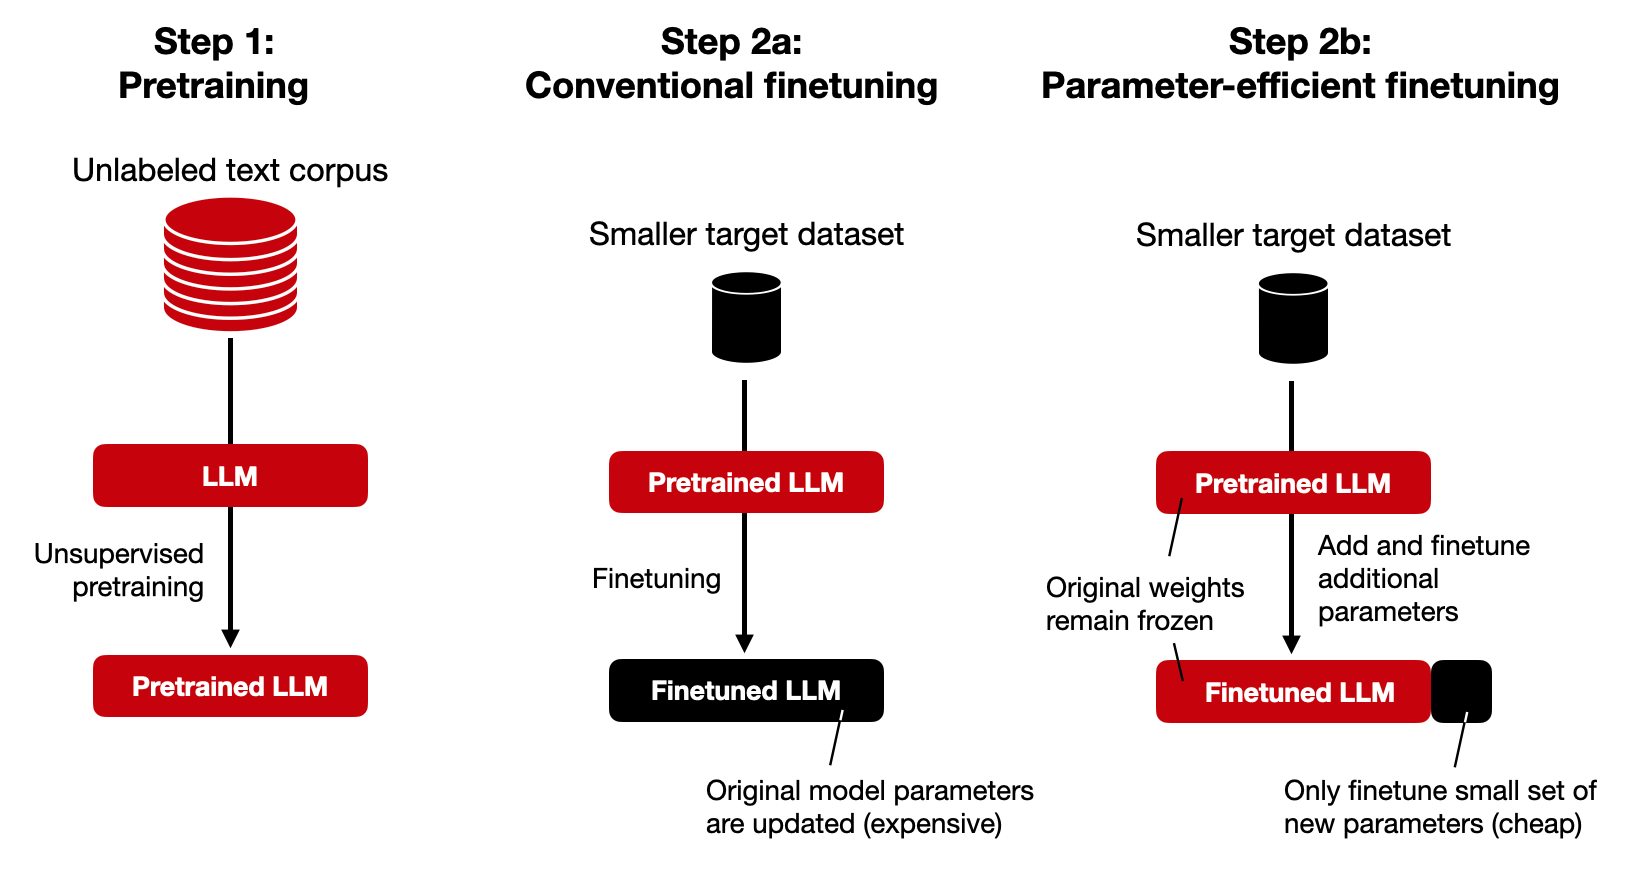
\includegraphics[width=.65\linewidth]{pictures/PEFT1.png}
    \caption[PEFT1]{process of PEFT  \cite{Raschka2023}}
    \label{fig:PEFT1}
\end{figure}

\begin{figure}[h!]
    \centering
    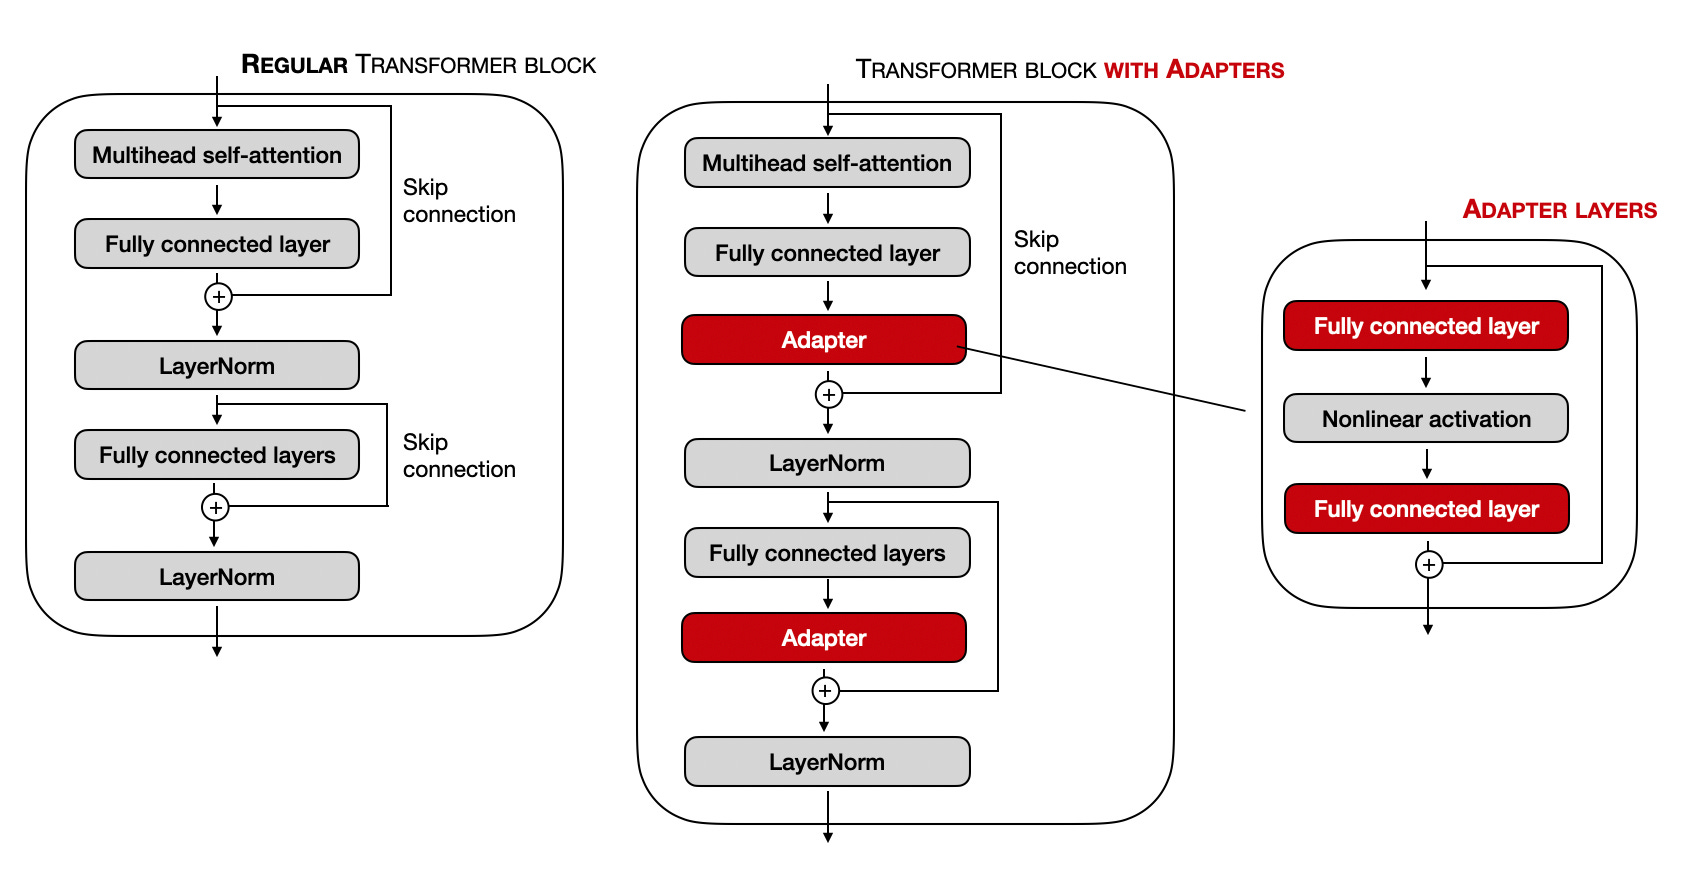
\includegraphics[width=.65\linewidth]{pictures/PEFT2.jpg}
    \caption[PEFT2]{process of PEFT (detailed) \cite{Raschka2023}}
    \label{fig:PEFT2}
\end{figure}




\subsection{Hugging Face}%Mohamad
Hugging Face is a pivotal platform in the field of natural language processing and machine learning, providing an extensive repository of pre-trained models along with tools for training, fine-tuning, and deploying models across various tasks. The platform is renowned for its implementation of state-of-the-art models, including those based on Transformer architectures like BERT, GPT, and their derivatives.

\textbf{Why Use Hugging Face?} The primary appeal of Hugging Face lies in its comprehensive ecosystem that simplifies the deployment of machine learning models. Here are several reasons why it is widely used:
\begin{itemize}
    \item \textbf{Accessibility of Pre-trained Models:} Hugging Face offers access to thousands of pre-trained models which are easily adaptable to a broad range of tasks without the need from scratch training.
    \item \textbf{Ease of Integration:} The platform supports various programming languages and frameworks, including Python, PyTorch, and TensorFlow, enabling seamless integration into existing projects.
    \item \textbf{Community and Support:} With a robust community of developers and researchers, Hugging Face facilitates collaboration and sharing of best practices, contributing to the continual improvement and extension of its model offerings.
\end{itemize}

\textbf{Benefits in Practical Applications:} Utilizing Hugging Face allows developers and researchers to reduce the time and resources required for model development dramatically. Specifically, the platform provides functionalities for:
\begin{itemize}
    \item \textbf{Fine-Tuning Pre-trained Models:} Users can fine-tune models on specific datasets, which is essential for tailoring the model's responses to the nuances of particular domains or tasks.
    \item \textbf{Experimentation:} The ease of accessing and modifying different models promotes rapid prototyping and experimentation, a valuable feature in the fast-evolving field of AI.
    \item \textbf{Deployment:} Hugging Face also offers solutions for easy deployment of trained models, which is beneficial for bringing AI applications to production.
\end{itemize}

\textbf{Application in Our Work:} In our research, we leverage Hugging Face to fine-tune pre-trained models specifically for analyzing Analyst Reports from MorningStar. This involves adapting state-of-the-art NLP models to comprehend and interpret complex financial texts, which is critical for extracting actionable insights and automating parts of the financial analysis process. The ability to fine-tune and deploy models efficiently with Hugging Face accelerates our research and application development, enabling a focused approach on model performance and application-specific adjustments rather than infrastructure and model maintenance.

\section{literature}%Jonas

As described in \cite{Zhao2024}, there are many different applications of LLMs, and specifically for analyst reports they can provide insights into subtle tone and sentiment to add value. However, at the moment there is only research on publicly available data such as Reddit \cite{Deng2023}. Furthermore, it has been shown that reports may have a small positive performance in the right market conditions \cite{Su2020}, but it is unclear whether only recommendations themselves can influence markets \cite{Brauer2018} and reports have no value at all \cite{Panchenko2007}. Thus, the herding factor may have an impact on stock performance \cite{Palmer2018}.
In \cite{Kim2023} they use LLMs to better interpret and analyze Korean financial analysts' reports.
In this paper, however, we use data from widely spread reports (from retail traders to professionals) on globally traded firms. We show that while analysts can barely outperform the current market, they provide comprehensive textual justifications that enable informed decisions. We use enhanced large language models to efficiently analyze the textual data, allowing a broad exploration of different pre-trained models to identify the subtle underlying sentiment and extract more value from the reports than the experts themselves.


\section{Approach}%Jonas
Our ultimate objective can be interpreted as a binary classification problem based on sentiment analysis. We use the textual data from the reports to predict whether the stock is a good investment or not. In order to do so we compare the performance of different models and configurations to find the best one. We also compare the performance of the models to the analysts' own predictions and other metrics from the report to create a baseline. In order to explore many different models and configurations, we use the parameter efficient fine-tuning approach. We use adapters to fine-tune the models and Hugging Face to access the pre-trained models. Even though literature has shown adapters to be more efficient while retaining the performance of the underlying model, we setup a preliminary experiment with the Stanford Sentiment Treebank v2 (SST2) data set for sentiment classification to validate our approach and compared the efficiency and performance of the models:
% here a table with results for

\begin{table}[h!]
    \centering
    \begin{tabular}{lcc}
    \toprule
     & \textbf{Fine-tuned LLM} & \textbf{Fine-tuned Adapter} \\
     \midrule
    {Training Runtime} & 1h 58m & \textbf{\textcolor{ForestGreen}{24m}} \\
    {Evaluating Accuracy} & \textbf{\textcolor{ForestGreen}{0.908}} & 0.902 \\
    {Evaluation Runtime} & 6.83s & \textbf{\textcolor{ForestGreen}{1.84s}} \\
    {Evaluation Loss} & 0.42 & \textbf{\textcolor{ForestGreen}{0.31}} \\
    \bottomrule
    \end{tabular}
    \caption{Comparison of Fine-tuned LLM and Fine-tuned Adapter}
    \label{tab:comparison}
    \end{table}


Therefore, we used PEFT to find the best performing setup and built a automated training and evaluation pipeline to efficiently explore the model landscape of Hugging Face.

\subsection{Model selection}%Jonas
Since our approach is centered around sentiment classification of financial reports, we allocated the most fitting pre-trained models from both worlds -- sentiment analysis and finance:


\noindent
\textbf{Sentiment:}
\begin{itemize}
\item \texttt{kwang123/bert-sentiment-analysis}
\item \texttt{siebert/sentiment-roberta- large-english}
\item \texttt{distilbert/distilbert-base- uncased-finetuned-sst-2-english}
\end{itemize}

\noindent
\textbf{Finance:}
\begin{itemize}
\item \texttt{ProsusAI/finbert}
\item \texttt{yiyanghkust/finbert-tone}
\item \texttt{bardsai/finance-sentiment-pl-fast}
\item \texttt{RashidNLP/Finance-Sentiment- Classification}
\item \texttt{ahmedrachid/FinancialBERT- Sentiment-Analysis}
\item \texttt{soleimanian/financial- roberta-large-sentiment}
\item \texttt{nickmuchi/sec-bert-finetuned- finance-classification}
\item \texttt{nickmuchi/deberta-v3-base- finetuned-finance-text-classification}
\end{itemize}

Among the finance subset, there are also models that are fine-tuned on the task of sentiment classification with finance related text data like the public available SEC filing reports.

\subsection{Adapter configuration}%Mohamad
Configuring adapters in machine learning models, particularly in Transformer architectures, allows for targeted modifications to model behavior while preserving the bulk of the pre-trained parameters. Adapters offer a flexible approach to fine-tuning, where specific components are added or adjusted to alter the model's functionality for specialized tasks. This section explores various adapter configurations and their applicability to our research.

\textbf{Adapter Configuration Options:} The configuration of adapters can vary widely depending on the desired outcome and the specific model architecture. Common configurations include altering the number of adapter layers, the size of the feed-forward networks, the non-linearity type, and the training strategy. The choice of configuration typically balances between computational efficiency and task-specific performance.

\textbf{Industry Standard and Our Usage:} For the industry, especially in areas involving complex sequence understanding like financial analysis, configurations that offer a good trade-off between performance and computational demand are preferred. In our work, we experimented with several adapter configurations to identify the most effective setup for analyzing financial reports.

\textbf{Adapter Configurations Used in Our Work:}
\begin{itemize}
    \item \textbf{LoRAConfig:} LoRA (Low-Rank Adaptation) employs rank decomposition to modify attention and feed-forward layers within a Transformer. By adjusting only a small subset of model parameters, LoRAConfig focuses on the adaptability of the model with minimal computational overhead.
    \item \textbf{UniPELTConfig:} The Universal Parameter-Efficient Learning of Tasks (UniPELT) is a strategy that integrates different types of parameter-efficient techniques. UniPELTConfig is designed to be flexible across a variety of tasks by leveraging multiple adaptation strategies simultaneously.
    \item \textbf{MAMConfig:} Model-Agnostic Meta-Learning (MAM) approach configures adapters for fast adaptation to new tasks. This configuration has proven particularly effective in settings where models need to quickly adjust to new data distributions or task requirements.
    \item \textbf{ConfigUnion (LoRAConfig, PrefixTuningConfig, SeqBnConfig):} This configuration combines LoRA, Prefix Tuning, and Sequence Bucketing strategies. Prefix Tuning involves prepending a sequence of trainable vectors to the input, while Sequence Bucketing adjusts the model based on sequence length. This union aims to leverage the strengths of each individual approach for enhanced overall performance.
\end{itemize}

\textbf{Performance Evaluation:} In our experiments, MAMConfig emerged as the best-performing configuration. Its effectiveness in adapting to the specific nuances of financial text in Analyst Reports from MorningStar has been particularly noteworthy. MAMConfig's ability to facilitate rapid learning and adaptation without extensive retraining makes it highly suitable for our application, leading to significant improvements in model precision and recall metrics.

In conclusion, the careful selection and configuration of adapters are crucial for optimizing the performance of fine-tuned models in specialized tasks. The diverse configurations we tested underscore the adaptability and potential of using adapters to enhance pre-trained models for specific domains like financial analysis.

\subsection{Exploration and Exploitation}%Jonas
Since running all possible combinations of configurations is intractable, we assume independence of our various parameters in our experimental setup and base our approach on exploration and exploitation. We explore all possible valid models and configurations and exploit the best ones in the next iteration. First we compare the different models, then we optimize for the best adapter configuration, and after that we search for the best text input. Finally, we compare our PEFT approach to fine-tuning the LLM itself.
All experiments are performed on the same data, using the same training and test split to ensure comparability, and we use the same evaluation metrics, training parameters and hyperparameters for all models. Everything is run on the same hardware.

\subsection{Evaluation} %Jonas
In order to validate learned models we compare predictions made from the model with previously separated test data. In this way, we can objectively evaluate them according to their predictive qualities. For this comparison, we utilize these fundamental principles:
\newline \textit{Sensitivity} or true positive rate ($\mathrm{TPR}$) is derived from the true positives $\mathrm{TP}$,  i.e., the correctly identified positives $\mathrm{P}$ from the test set:
$
\mathrm{TPR}=\frac{\mathrm{TP}}{\mathrm{P}}
$
\newline \textit{Specificity} or true negative rate ($\mathrm{TNR}$) is derived from the true negatives $\mathrm{TN}$,  i.e., the correctly identified negatives $\mathrm{N}$ from the test set:
$
\mathrm{TNR}=\frac{\mathrm{TN}}{\mathrm{N}}
$

\begin{figure}[h!]
    \centering
    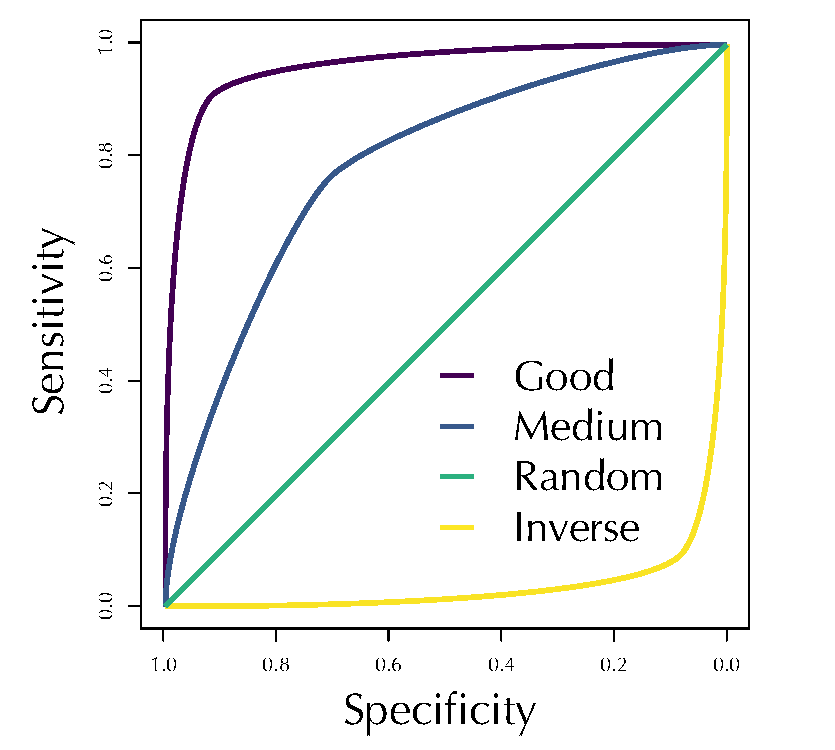
\includegraphics[width=.85\linewidth]{pictures/ROC.pdf}
    \caption[ROC explanation]{Exemplary receiver operating curves for  a \textit{good, medium, random} and \textit{inverse} model fit. The perfect score would be 1.0 on each dimension -- specificity and sensitivity.}
    \label{fig:exroc}
    \end{figure}

By plotting both the sensitivity and specificity in relation for various threshold values, we obtain the so called Receiver Operating Characteristic (ROC) curve. For the results of both measures 1.0 is the optimum, and if the curve is the diagonal, we observed a random process.  In Figure~\ref{fig:exroc}, we can see some common examples of curves. In order to further summarize these evaluations, we can calculate the Area Under the Curve (AUC) to rank the models. Again, a value of 0.5 indicates a random process.
The reason we use ROC rather than accuracy, precision, recall and f1 score is that ROC is a more comprehensive metric that provides a more detailed view of model performance. In addition, ROC curves make it easier to compare the performance of different models across all classification thresholds. This also makes it more robust to class imbalance, which is very important for inherently unbalanced data such as financial markets, which often follow trends. It also helps to understand how the performance of the model changes with different classification thresholds, which can be crucial for decision making in different conditions where the cost of false positives and false negatives can vary. \cite{Hastie2009}  \cite{Kauermann2021}  \cite{Russell2021}



\section{Results}%Jonas
In this section we present the results of our experiments. We compare the models with classical approaches based on the analysts' forecasts themselves and other metrics from the report to establish a baseline. We present the results of our model training in three steps: First, we compare the different models, then we optimize the best adapter configuration, and finally we search for the text input that provides the highest predictive power. We also directly fine-tune the underlying model to see if PEFT loses significant predictive power. We also use feature attribution via CAPTUM to gain insight into the models and provide an overview of training time, runtime and number of parameters.

\subsection{Benchmarking}%Jonas
In order to evaluate our models accurately, we first create a benchmark based on the analysts' own predictions. We use the analysts' \texttt{FairPrice} to create binary predictions and use them  as input for a logistic regression model as a first benchmark. We also use all the categorical (and ordinal) information from the reports as input for an gradient boosted tree model (XGBoost) as a benchmark: \texttt{Rating, AuthorName, Uncertainty, EconomicMoat, CostAllocation, FinancialStrength, Sector, Exchange, Prediction}. We assume that certain authors might be better than others, and that the uncertainty, economic moat, cost allocation and financial strength might be valid indicators of a firms success. We also assume that the sector and exchange might have an impact on the stock performance. We use the same training and test split as for the LLMs and the same evaluation metrics. The results are shown in Figure~\ref{fig:Zeroexp}.

\begin{figure}[h!]
    \centering
    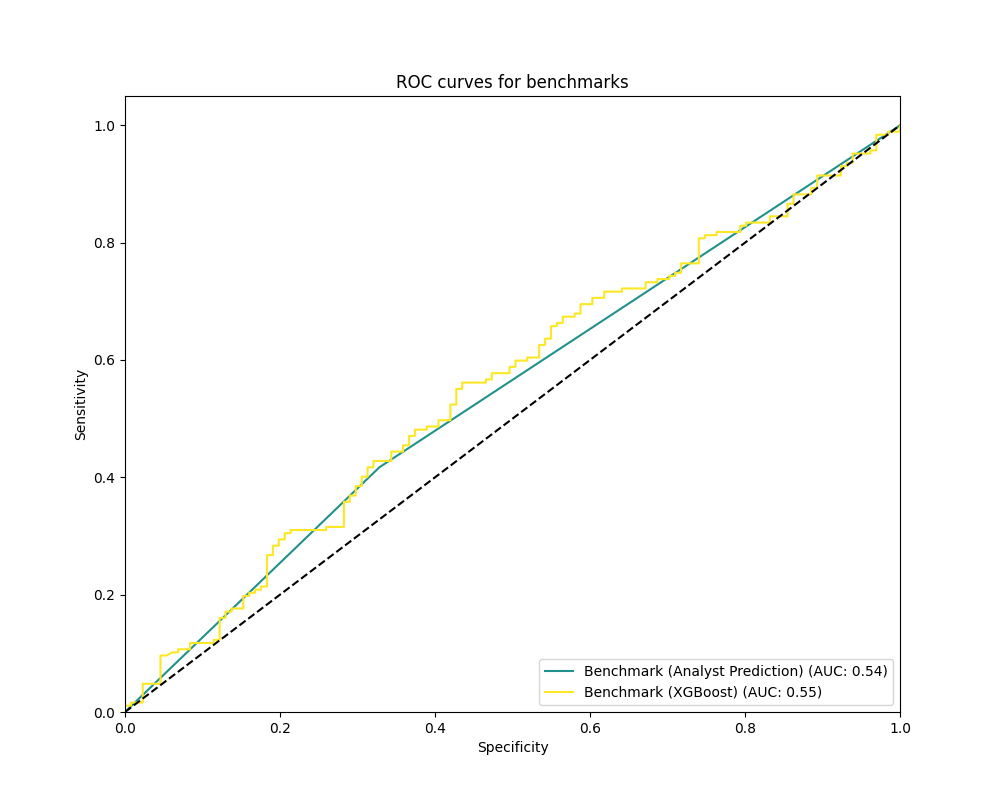
\includegraphics[width=.85\linewidth]{../3. evaluation/roc_curves/Zero Experiment.png}
    \caption[First Experiment]{Benchmark Experiment}
    \label{fig:Zeroexp}
\end{figure}

The results show that neither the analysts nor the XGBoost model can outperform randomness -- it only reproduces the current distribution of the market (trend following). This is a strong indication that the reports themselves may not contain any valuable information.

\subsection{Models in comparison}%Jonas
Our approach assumes that all changes in our experiments are independent and that the results are comparable. As first step we compare the different models on the same adapter configurations and text inputs to find the best one.

\begin{figure}[h!]
    \centering
    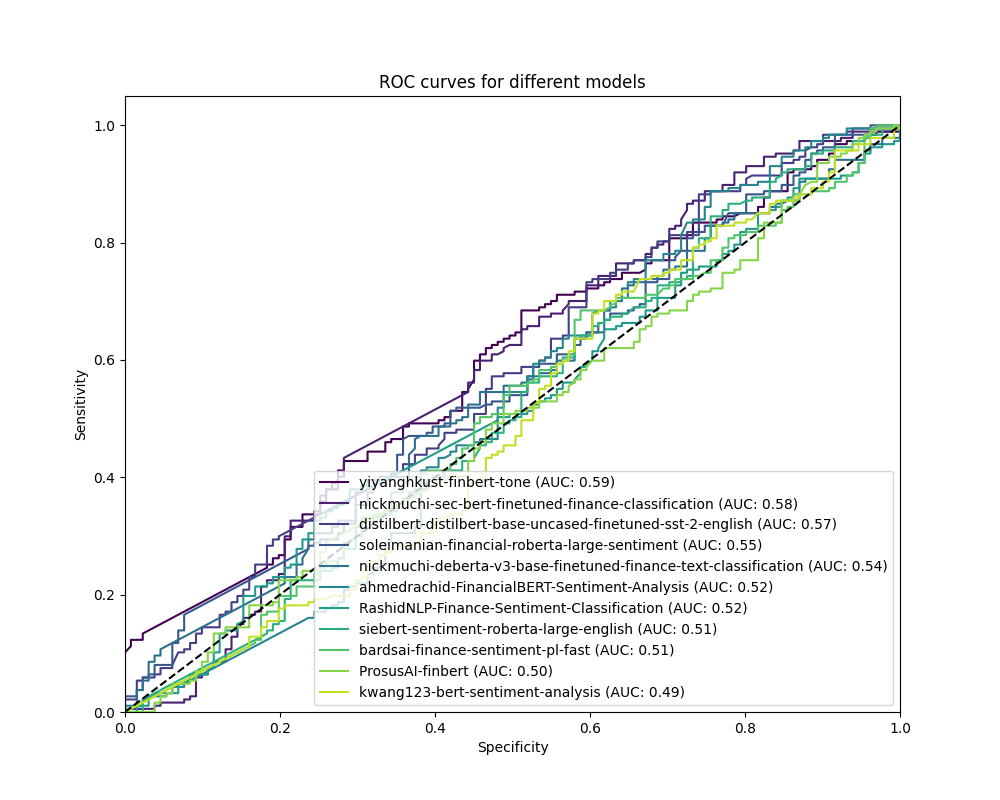
\includegraphics[width=.85\linewidth]{../3. evaluation/roc_curves/First Experiment.png}
    \caption[First Experiment]{First Experiment}
    \label{fig:Firstexp}
\end{figure}
We continue for the two best models (both trained on financial sentiment data) and compare the best adapter configurations found in literature:

\begin{figure}[h!]
    \centering
    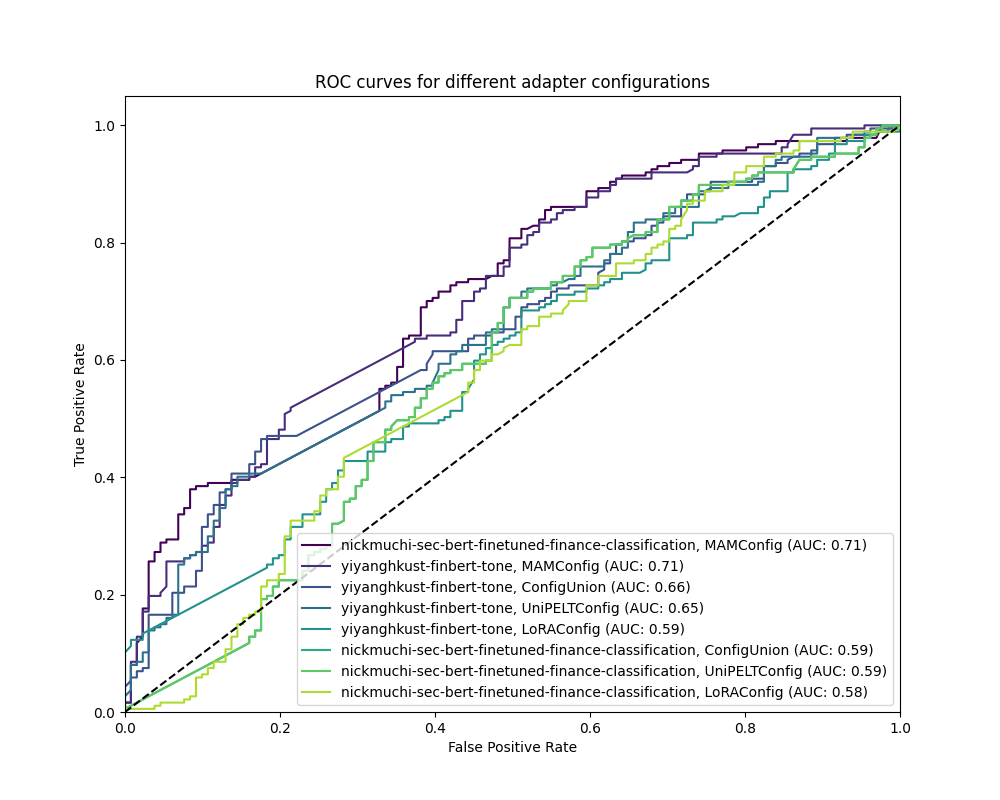
\includegraphics[width=.85\linewidth]{../3. evaluation/roc_curves/Second Experiment.png}
    \caption[Second Experiment]{Second Experiment}
    \label{fig:Secondexp}
\end{figure}

Next to \texttt{AnalystNoteList} we also explore \texttt{BullsList, BearsList, ResearchThesisList, MoatAnalysis, RiskAnalysis, CapitalAllocation, Profile}, and  \texttt{FinancialStrengthText} as input data. We find that \texttt{FinancialStrengthText} as a concise summary provides the best predictive power.

\begin{figure}[h!]
    \centering
    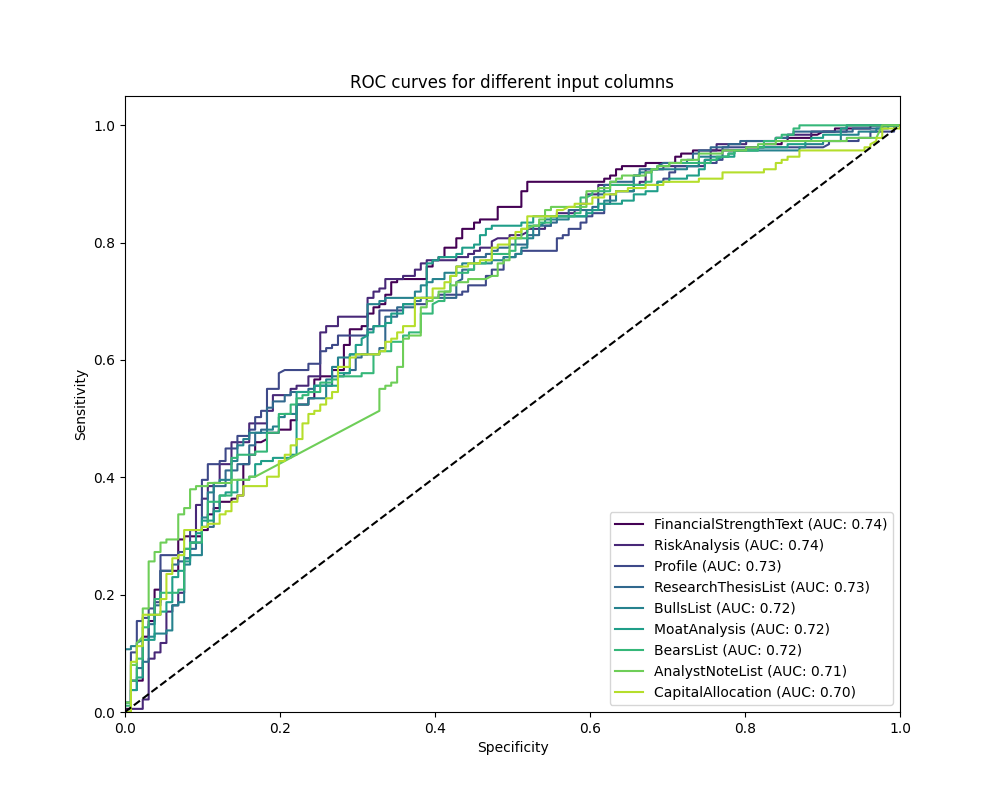
\includegraphics[width=.85\linewidth]{../3. evaluation/roc_curves/Third Experiment.png}
    \caption[Third Experiment]{Third Experiment}
    \label{fig:Thirdexp}
\end{figure}

Finally, we use the best combination found to directly fine tune the underlying model. This leads to only a small improvement of 0.0031 AUC and the training time was roughly the same, but the number of parameters could be drastically decreased from 110 million to 23 million.

\begin{figure}[h!]
    \centering
    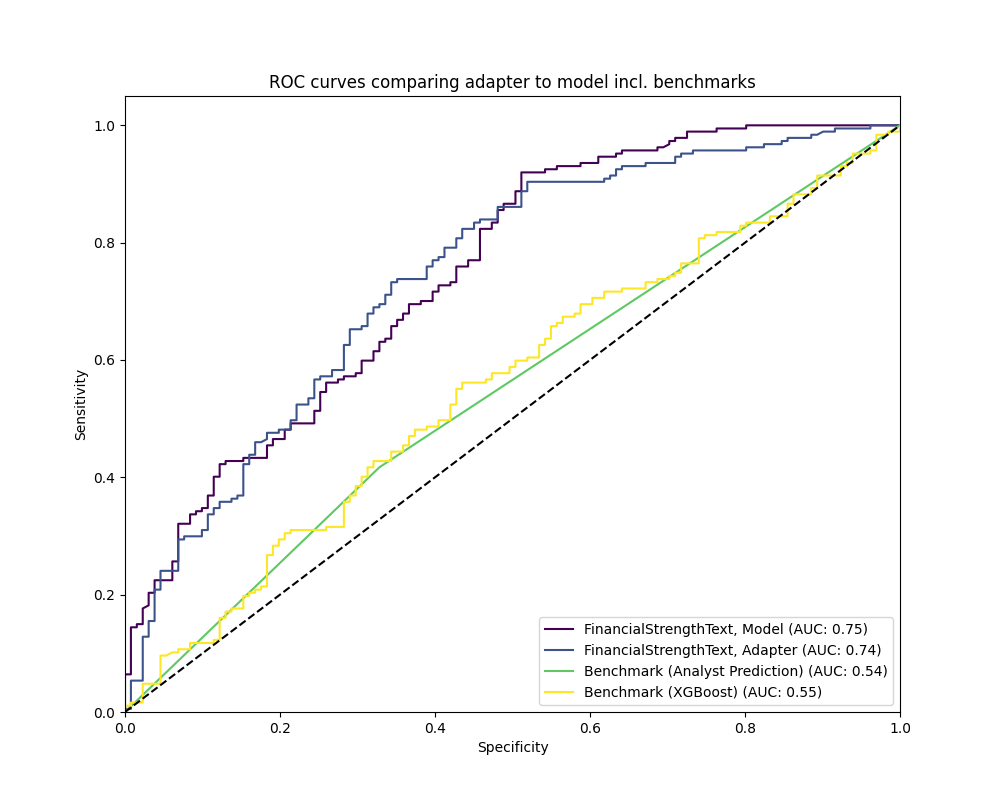
\includegraphics[width=.85\linewidth]{../3. evaluation/roc_curves/Fourth Experiment.png}
    \caption[Fourth Experiment]{Fourth Experiment}
    \label{fig:Fourthexp}
\end{figure}

While there is no overall cutoff value and it highly depends on the specific application, with values above 0.7 \cite{Hosmer2013}, we reached a robust predictive quality.

\subsection{Insights via CAPTUM}%Mohamad
What are the models using as input? Use CAPTUM and quickly describe the gradient approach to obtain feature attribution. \cite{Kokhlikyan2020}

CAPTUM, which derives from the Latin word for "understanding," is a model interpretability library for PyTorch developed by Meta AI. It provides a comprehensive suite of algorithms designed to provide insights into the data features that most influence machine learning models' predictions. This tool is crucial for validating model behaviors, ensuring fairness, and debugging in complex machine learning systems.

\textbf{Captum.AI} offers a range of interpretability methods, but a prominent approach within this library involves gradient-based techniques for feature attribution. These methods compute the gradient of the output with respect to the input features to determine how much each feature contributes to the output prediction. The premise is that the gradient of a feature indicates the direction and magnitude by which a slight change in the feature would alter the model's output.

\textbf{Gradient Approach for Feature Attribution:} The gradient-based methods, such as Integrated Gradients, are particularly popular. This method accumulates gradients along the path from a baseline input (typically representing the absence of a feature) to the actual input, providing a more comprehensive picture of feature importance across different contexts within the input space.

Using CAPTUM, researchers and developers can gain deeper insights into the workings of their models, enabling a clearer understanding of decision-making processes and facilitating improvements in model design and function. In our work, we employ CAPTUM to analyze and validate the feature attributions of our fine-tuned models on financial texts from Analyst Reports by MorningStar, ensuring that our models make decisions based on relevant and justifiable information.



\subsection{Training analysis}%Mohamad
Show some plots about runtime and training time. Compare with Loss, Accuracy etc

\section{Conclusion}
Wrap it up and discuss the results. What are the implications? What are the limitations?
\bibliographystyle{IEEEtran}
\bibliography{report}

\end{document}
